\def \typIntro {Typesystem Introduction}
\section{Introduction}

\begin{frame}
  \frametitle{Are Typesystems Useful?}
  
  \begin{itemize}
    \item Advent of DSLs and DSL tools
    \item Writing languages is easy, even for complex domains
    \item Complex languages $\Rightarrow$ complex constraint checking
    \item Most languages have a concept of \textbf{types}: reusable building
    blocks for constraints
  \end{itemize}
\end{frame}

\begin{frame}
   \tableofcontents
\note{
  In this presentation:
  \begin{itemize}
    \item Compare different type system approaches
    \item Case study: form based editing of entities
    \item Xtext as DSL development environment
  \end{itemize}}
\end{frame}

\begin{frame}[fragile]
  \frametitle{\typIntro}
  \begin{columns}[T]
        \column{.6\textwidth}
        % Generator: GNU source-highlight, by Lorenzo Bettini, http://www.gnu.org/software/src-highlite
\begin{tabular}[t]{l}
\noindent
\mbox{}name\ :\ \textbf{\textcolor{Plum}{string}}; \\
\mbox{}greeting\ =\ \textcolor{RoyalBlue}{"{}Hello\ "{}}\ +\ name\ +\ \textcolor{RoyalBlue}{"{}!"{}}; \\
\mbox{}
\end{tabular}

        \column{.4\textwidth}
        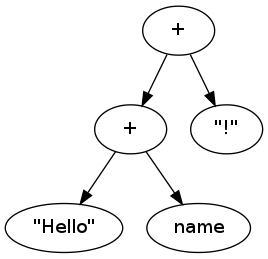
\includegraphics[scale=0.45]{img/ast1.png}
  \end{columns}
  \pause
  Common type system tasks:

  \begin{itemize}
    \item Assign types to language elements
    \item Infer types of complex expressions
    \item Is a type conformant to another type?
  \end{itemize}
  \note{
     \begin{itemize}
       \item Static type checking example
     \end{itemize}
     assigning fixed types to certain language elements \\
     conformance: subtype relationships
   }
\end{frame}